\documentclass[11pt,a5paper,landscape]{article}

\usepackage{main}
\usepackage{exercices}

% --------------------------------------------------
% Informations du document
% --------------------------------------------------
\renewcommand{\typedocument}{Exercices}
\renewcommand{\classe}{6e}
\renewcommand{\titre}{Exercices - Mouvement et vitesse}

\begin{document}
\begin{multicols*}{2}

% ----- Exercice 1 -----

\exercice{Vitesse moyenne}
\begin{enumerate}
    \item Si une voiture roule à la vitesse de 50 kilomètres par
heure (km/h), quelle distance parcourt-elle en une heure ?
    \item Une voiture relie Limoges à Paris en 5h. La distance
Limoges-Paris est de 400 km. Calculez la vitesse de la
voiture en kilomètre par heure (km/h).
    \item Les escaliers de la maison d'Oscar font 10 mètres et il met 5 secondes à les monter. Quelle est sa vitesse moyenne en mètres par seconde (m/s) ?
\end{enumerate}

% ----- Exercice 2 -----

\exercice{Référentiel}
Les escalators parcourent 15m en 10s.

\begin{center}
    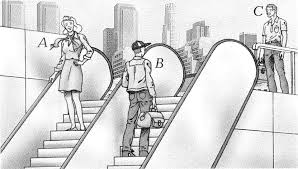
\includegraphics[width=6cm]{images/escalators mouvement.jpg}
\end{center}

\begin{enumerate}
        \item Par rapport au référentiel terrestre, qui est en mouvement ?
        \item Quelle est la vitesse de A par rapport à C ? et à B ?
\end{enumerate}

\columnbreak

% ----- Exercice 3 -----

\exercice{Trajet en vélo}
Timothée se rend au collège en vélo. Il part de chez lui à 7h30 et arrive au collège à 8h, en ayant fait 4km.
\begin{enumerate}
    \item Quelle est la durée du trajet en minute ? et en heure ?
    \item Calculer la vitesse moyenne en km/h.
    \item Lorsqu’il est en retard, son papa l’emmène en voiture. Le trajet dure 15 minutes. Quelle est la vitesse moyenne en km/h?
\end{enumerate}

% ----- Exercice 4 -----

\exercice{Course entre amis}
Mathis court le 100m en 16s et Nathan court le 60m en 12s. Puisqu’il a fini avant, Nathan pense qu’il a été plus rapide.
\begin{enumerate}
    \item Calculer la vitesse de Mathis en m/s.
    \item Calculer la vitesse de Nathan en m/s.
    \item Nathan avait-il raison ?
\end{enumerate}

% ----- Exercice 5 -----

\exercice{km/h et m/s}
\begin{enumerate}
    \item Convertir une heure en secondes.
    \item Convertir un km en m.
    \item Si je fais un kilomètre en une heure, combien de mètres je fais en combien de secondes ?
    \item Combien vaut 1 km/h en m/s ?
\end{enumerate}

\end{multicols*}
\end{document}